\chapter{Conceitos Fundamentais}

Este capítulo apresenta os conceitos fundamentais que servem de base para o desenvolvimento da presente pesquisa. As primeiras seções descrevem os fundamentos do aprendizado de máquina e visão computacional, as seções seguintes aprofundam os conceitos amplamente utilizados na pesquisa sobre redes neurais e a geração de dados sintéticos, por fim a última seção trás luz sobre a explicabilidade de modelos caixa preta e se aprofunda nas técnicas importantes para a avaliação de modelos de imagens.

\section{Aprendizado de máquina}

A abordagem de aprendizagem de máquina (do inglês \textit{machine learning}), é fundamental para a resolução de diversos problemas por meio do reconhecimento de padrões \cite{bishopPatternRecognitionMachine2006}. 
Em essência o objetivo do reconhecimento de padrões está na descoberta automática de relações entre as diferentes características de um determinado fenômeno, de modo que essas relações possam ser utilizadas para a tomada decisão em diversos tipos de atividades como: previsão do tempo, diagnósticos médicos, determinação do preço de um ativo e o reconhecimento de indivíduos.

Para algumas tarefas, o reconhecimento de padrões tem a premissa de que as relações entre as características de um evento e o fenômeno resultante podem ser modeladas matematicamente do seguinte modo $f(x) = y$, em que $f$ é o modelo real que deve ser aprendido, e geralmente não conhecemos, $x$ são as condições observáveis do nosso evento e $y$ o fenômeno causado - comumente definido como variável alvo ou variável dependente.

Deste modo, a tarefa de aprendizagem de máquina se resume em inferir um modelo $h(x) = y$, onde $h$ é um modelo hipotético da realidade que quando bem definido pode-se aproximar do modelo real $f$.

Para que possamos inferir este modelo hipotético $h$, se faz necessária a construção de um conjunto de dados $X$ que será divido em um \textbf{conjunto de treinamento} e outro \textbf{conjunto de teste}.
Em alguns casos, pode ser necessário uma etapa de \textbf{extração de características} que serão de fato utilizadas para a construção do modelo, por exemplo, na construção de modelos de classificação de imagens.
O conjunto de treinamento é aplicado a fase de aprendizado, onde os parâmetros e regras do modelo serão inferidas. Já o conjunto de teste, será utilizado para uma etapa de validação, esta etapa tem por objetivo verificar o quão distante do modelo real $f(x)$ está o modelo $h(x)$.

A tarefa de aprendizagem de máquina pode ser classificada em diferentes tipos sendo: aprendizado supervisionado, aprendizado não supervisionado e aprendizado por reforço \cite{bishopPatternRecognitionMachine2006}.

\subsubsection{Aprendizado supervisionado}

O aprendizado supervisionado é definido quando para o fenômeno a ser modelado temos além das características a variável alvo relacionada a cada instância do nosso conjunto de dados. Os problemas resolvidos pelos modelos supervisionados podem ser divididos em problemas de regressão e classificação.

Os problemas de regressão são caracterizados pela modelagem de variáveis alvo numéricas, por exemplo, preços de ativos, temperatura, volume de chuva e idade.
Já os problemas de classificação investigam a relação entre as características e as diferentes classes de uma determinada população de estudo, como classificar corretamente imagens médicas para produção de diagnósticos.
Dada a natureza do presente trabalho, é importante nos debruçarmos mais sobre os conceitos relacionados ao problema de aprendizado supervisionado para classificação de instâncias, para isso, a seção \ref{secao:algoritmos-classificacao} se aprofundará em mais detalhes sobre estes modelos e seus métodos de avaliação.

\subsubsection{Aprendizado não supervisionado}

Os modelos de aprendizado não supervisionados consistem em modelos de aprendizagem de máquina que tem por objetivo a aplicação de técnicas de agrupamento no conjunto de dados.
Note que neste caso, não temos uma variável alvo a ser modelada.
Estes agrupamentos podem ser utilizados em diferentes contextos para a tomada de decisão, de modo que um tratamento em específico pode ser atribuído a cada grupo com base em suas características próprias.
Nesta classe de problema, diferentes algoritmos são empregados como agrupamento hierárquico, \textit{K-Means}, \textit{K-Nearest Neighbors} e \textit{DBSCAN}. Além disso, as técnicas de avaliação do modelo também são específicas como o coeficiente de silhueta e escores baseados em informação mútua.

\subsubsection{Aprendizado por reforço}

Os modelos de aprendizado por reforço, buscam a partir da definição de um ambiente que possui diferentes estados, encontrar via tentativa e erro a sequência de ações em cada estado que maximizam uma recompensa pré-definida, de modo que cada ação tomada possa afetar a próxima cadeia de estados seguinte \cite{bishopPatternRecognitionMachine2006}.



\section{Algoritmos supervisionados de classificação} 
\label{secao:algoritmos-classificacao}

Os modelos de classificação fazem parte do paradigma de aprendizado supervisionado, com aplicação na descoberta de relações entre as diferentes características de uma instância e sua classe atribuída. Assim como outros modelos de aprendizagem de máquina, os modelos de classificação, em geral, também possuem um \textbf{algoritmo de aprendizado} para a inferência de suas regras e parâmetros.

Existem diversos tipos de modelos que assumem diferentes premissas sobre a natureza do problema a ser resolvido e que podem ser utilizados para tarefa de classificação, desde modelos mais simples e paramétricos como a regressão logística até modelos não paramétricos mais complexos como \textit{XGBoost}, \textit{CatBoost} e redes neurais artificiais (RNA).

Apesar de cada modelo possuir suas próprias características, a resolução de problemas de classificação possui um arcabouço bem definido e agnósticos aos modelos de técnicas de avaliação de performance. As principais métricas que são utilizadas neste arcabouço são explicadas em detalhes a seguir.

\subsection{Métodos de avaliação}

Os métodos de avaliação de modelos de classificação passam pela interpretação da matriz de confusão. Nesta matriz, são apresentados os erros e acertos do modelo para as diferentes classes que estão sendo modeladas, sendo que a aplicação se dá tanto para modelos de classificação binária e também para modelos de classificação multi-classe.

Por meio do esquema da matriz de confusão apresentado na figura \ref{fig:matriz-de-confusao}, é possível quantificar a quantidade de casos classificados corretamente e erroneamente pelo modelo levando em consideração as classificações verdadeiras positivas (TP), verdadeiras negativas (TN), falsas positivas (FP), também conhecidas como erro do tipo I e falsas negativas (FN), também definidas como erro do tipo II.
Desta matriz pode-se derivar diversas métricas que resumem a qualidade do modelo empregado para a tarefa de classificação como acurácia, sensibilidade, precisão, especificidade e F1.

\begin{figure}[htbp]
	\centering
	\caption{Matriz de confusão: a matriz de confusão pode ser aplicada a problemas de classificação binário ou multi-classe, por meio desta matriz, pode-se derivar diversas métricas que auxiliam a compreensão da performance do modelo. }
		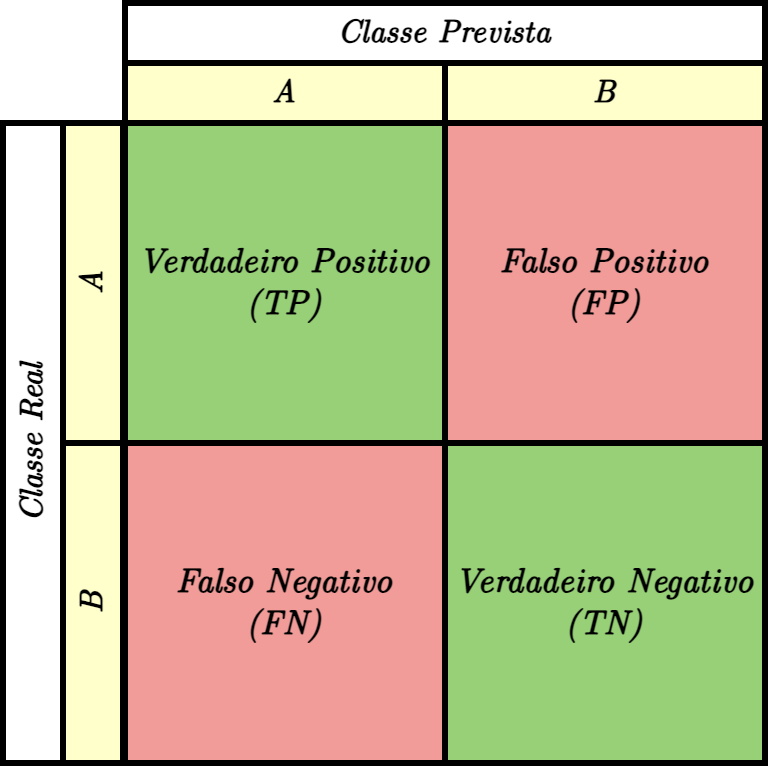
\includegraphics[scale=.25]{imagens/matriz-de-confusao.png}
	\label{fig:matriz-de-confusao}
  \source{Alexandre Farias, 2024}
\end{figure}

\subsubsection{Acurácia}

A acurácia mede no quadro geral a quantidade de acertos do modelo, levando em consideração todas as classes, pode se ler a acurácia como a proporção de casos classificados corretamente, a métrica vai de 0 a 1, quanto maior melhor é o modelo. A medida é definida pela seguinte fórmula:

\begin{equation}
    \text{Acurácia} = \frac{TP + TN}{TP + TN + FP + FN}
\end{equation}

\subsubsection{Sensibilidade}

A sensibilidade, também conhecida por revocação, mede a quantidade de casos classificados corretamente de uma classe em específico, esta medida contribui para a compreensão do quão bem um modelo consegue detectar a respectiva classe, a métrica vai de 0 a 1, quanto maior, melhor é a capacidade do modelo de detectar a classe em questão, sua fórmula é dada por:

\begin{equation}
    \text{Sensibilidade} = \frac{TP}{TP + FN}
\end{equation}

\subsubsection{Precisão}

A precisão é uma medida da proporção de instâncias classificadas corretamente de uma determinada classe, essa métrica nos ajuda a entender a proporção das instâncias classificadas pelo modelo que realmente pertencem a classe predita, a métrica vai de 0 a 1, quanto maior, mais confiança temos nas previsões do modelo, sua fórmula é dada por:

\begin{equation}
    \text{Precisão} = \frac{TP}{TP+FP}
\end{equation}

\subsubsection{F1}

A medida F1 é a média harmônica entre a precisão e a sensibilidade, esta medida nos da um resumo da performance do modelo mais adequado para cenários onde há desbalanceamento de classes, dado que a acurácia é sensível a este equilíbrio e pode levar a conclusões equivocadas, por exemplo, em um conjunto de dados com um proporção de classes de 100:1, classificar todas as instâncias como a classe majoritária leva a uma acurácia de praticamente 99\%, no entanto a precisão do modelo é degradada. A fórmula da medida F1 é dada da seguinte maneira:

\begin{equation}
    F_{1} = 2\frac{\text{Precisão} * \text{Sensibilidade}}{\text{Precisão} + \text{Sensibilidade}}
\end{equation}

\subsubsection{Área sob a curva ROC}

A medida \textit{area under curve receiver operating characteristic} (AUCROC) é uma medida resumo da curva que leva em consideração a sensibilidade e a taxa de falsos positivos do modelo (FPR), comumente utilizada em modelos de classificação binário, onde podemos estabelecer uma classe sendo positiva e outra negativa, para calcular os diferentes pontos da curva, basta variar o limiar de probabilidade de classificação para o modelo e calcular as medidas de sensibilidade e FPR em cada ponto.
A taxa de falsos positivos é simplesmente a quantidade de instâncias classificadas incorretamente como pertencendo a classe positiva sob o universo de instâncias da classe negativa sendo $FPR = \frac{FP}{N}$, pode-se deduzir diretamente da taxa FPR que seu mínimo é 0, quando o modelo não classifica nenhuma instância negativa incorretamente e seu máximo é 1, quando o modelo classifica todas as instâncias negativas incorretamente. A figura \ref{fig:aucroc} ilustra o exemplo de um classificador binário, a linha pontilhada indica a performance teórica esperada de um classificador aleatório, dado que ambos os eixos vão até 1, sendo a medida F1 a área sob a curva, é direto que seu mínimo e máximo são respectivamente 0 e 1, sendo que quanto maior a métrica, melhor é a performance do classificador.
A curva AUCROC é sensível ao desbalanceamento do conjunto de dados, pois com pouquíssimas amostras na classe minoritária a sensibilidade e a taxa de falsos positivos podem levar a uma interpretação incorreta sobre a performance do modelo, dado que ambas as medidas são sensíveis ao balanceamento das classes.

\begin{figure}[htbp]
	\centering
	\caption{Exemplo de curva ROC: a linha pontilhada representa um modelo que classifica as instâncias aleatoriamente, a linha contínua representa um classificador que possui uma performance melhor que o \textit{baseline} aleatório.}
		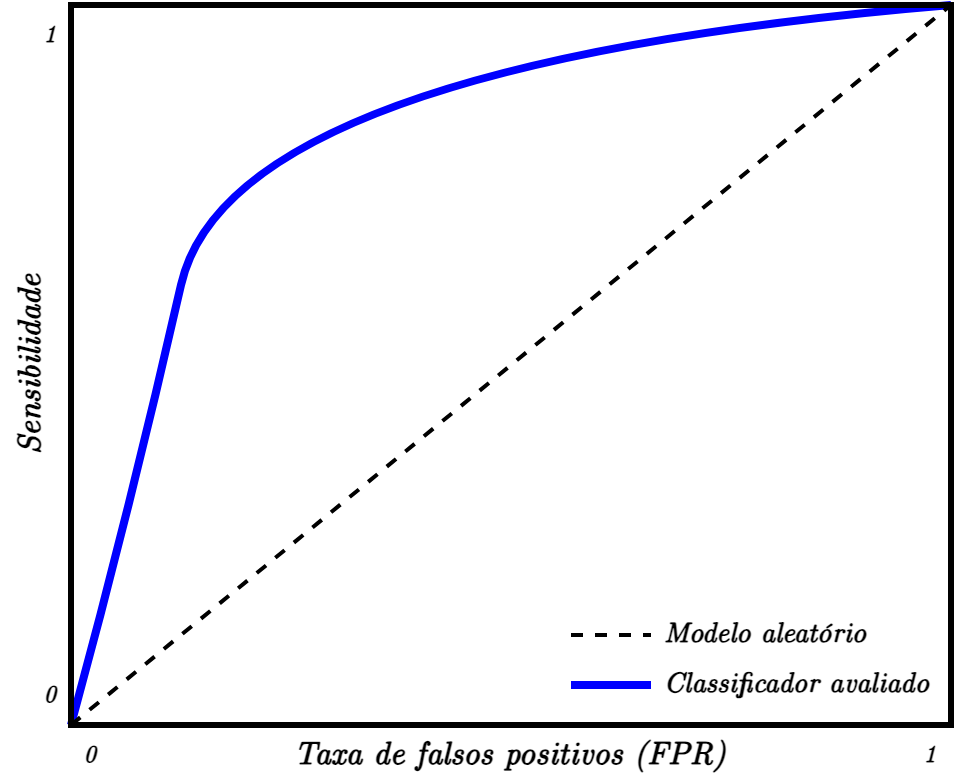
\includegraphics[scale=.25]{imagens/auroc.png}
	\label{fig:aucroc}
  \source{Alexandre Farias, 2024}
\end{figure}

\subsubsection{Área sob a curva de Precisão e Sensibilidade}

A área sob a curva de precisão e sensibilidade (PRAUC) permite avaliar a performance do modelo em diferentes limiares de classificação em problemas de classificação binários.
A utilização desta curva é recomendada para avaliar modelos treinados em conjuntos de dados desbalanceados, pois enquanto a medida de sensibilidade nos da a probabilidade de detecção da classe positiva, a medida de precisão nos dá uma visão sobre a probabilidade de uma previsão da classe positiva estar correta. A figura \ref{fig:prcurve} mostra o exemplo da avaliação de um classificador utilizando a curva PR, a precisão esperada de um modelo aleatório é de 50\%. A medida PRAUC tem como valor mínimo 0 e valor máximo 1, onde quanto maior, melhor.

\begin{figure}[htbp]
	\centering
	\caption{Exemplo de curva PR: a linha pontilhada representa a performance teórica de um classificador aleatório que serve como \textit{baseline}, já linha contínua representa a performance de um classificador que possui uma área sob a curva maior, sendo consequentemente melhor que o \textit{baseline}}
		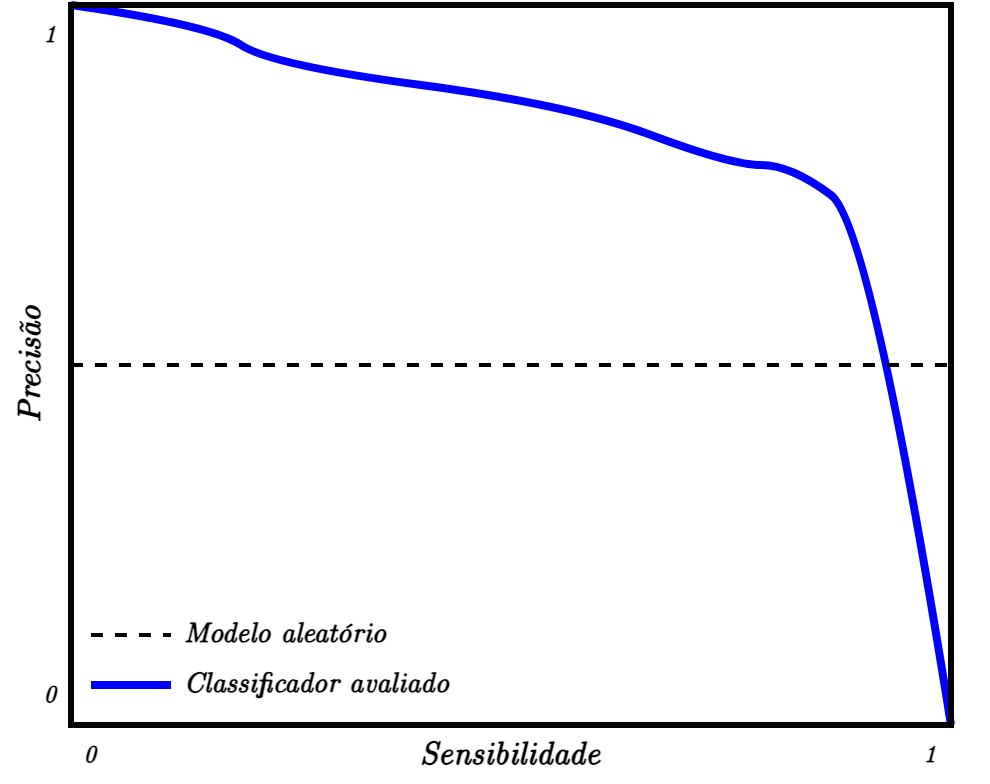
\includegraphics[scale=.25]{imagens/prcurve.png}
	\label{fig:prcurve}
  \source{Alexandre Farias, 2024}
\end{figure}

\section{Visão Computacional}

A visão computacional é um ramo da computação...

\section{Redes neurais artificiais (RNA)}

As redes neurais artificiais (RNA) fazem parte de um paradigma de modelos conexionistas, sua inspiração é a forma como o cérebro humano processa dados e os converte em informações relevantes por meio dos neurônios e suas interconexões. Segundo \citeonline{haykinNeuralNetworksLearning2009} as RNAs são modelos que possuem diferentes capacidades e propriedades úteis como: não-linearidade, adaptabilidade, respostas probabilísticas, informação contextual, tolerância a falhas, capacidade de computação paralela e uniformidade.

A não-linearidade das RNAs está associada ao fato de possuir uma arquitetura flexível, podendo ser utilizada para a construção de modelos de regressão e classificação, como os primeiros modelos de neurônios propostos em \citeonline{rosenblattPerceptronProbabilisticModel1958}. Adicionando camadas ocultas de computação, pode-se construir a rede \textit{Multilayer Perceptron} (MLP), também conhecida como \textit{feed-forward neural network}. A figura \ref{fig:perceptron} ilustra a arquitetura destes modelos.

A adaptabilidade se dá pelo fato do ponderamento adaptável dos pesos sinápticos das conexões existentes entre as unidades de computação, os neurônios. Estes pesos podem ser ajustados por meio de algoritmos como \textit{backprogapation} utilizando técnicas de gradiente descendente que buscam minimizar o erro do modelo em um determinado problema de reconhecimento de padrões.

Como apresentado na figura \ref{fig:perceptron} (a), os neurônios realizam uma combinação linear dos dados da camada de entrada e aplicam uma função $\phi$ a este resultado. Ao determinar funções de ativação específicas como a função sigmoide, a rede neural artificial pode fornecer como saída probabilidades úteis para a classificação de instâncias.

\begin{figure}[htbp]
	\centering
	\caption{Arquitetura de um neurônio e da rede multilayer perceptron: (a) Um neurônio artificial recebe dados em sua entrada e realiza uma combinação linear com base em seus pesos sinápticos, em sequência a função de ativação é aplicada a este resultado. (b) A rede MLP é caracterizada pela utilização de uma ou mais camadas ocultas com múltiplos neurônios.}
		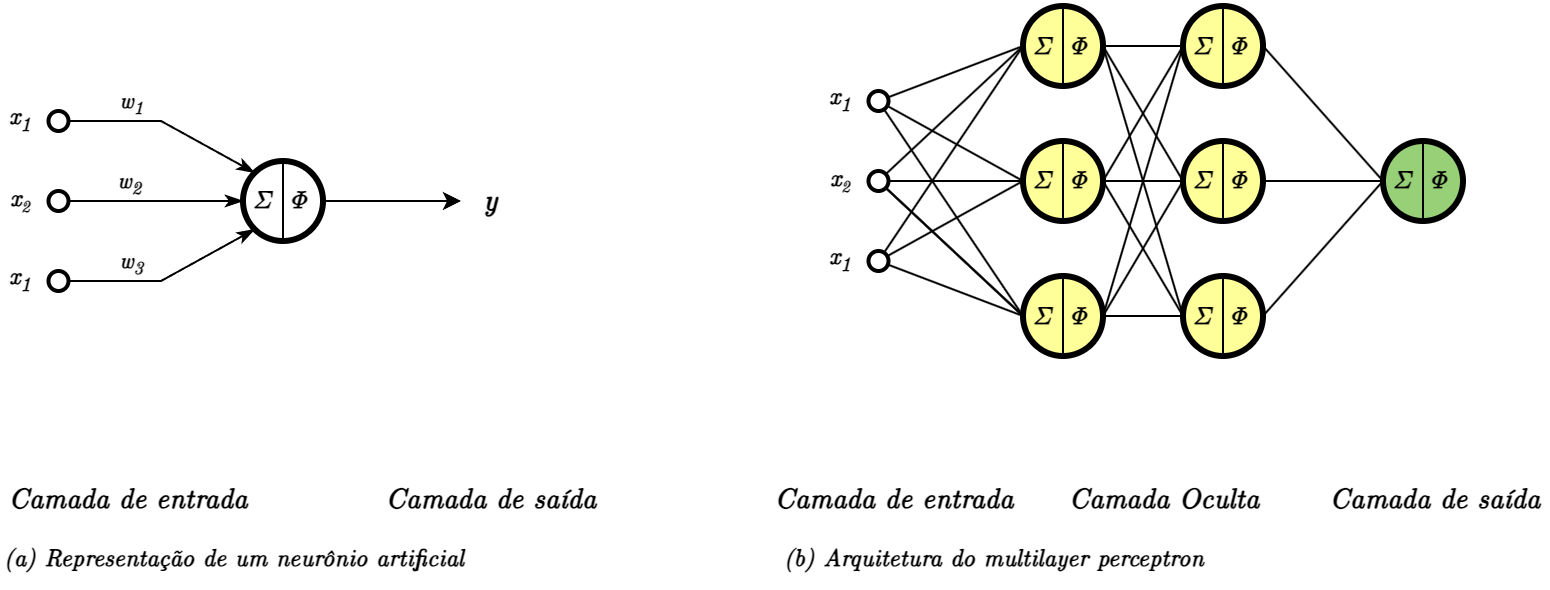
\includegraphics[scale=.25]{imagens/perceptron.png}
	\label{fig:perceptron}
  \source{Alexandre Farias, 2024}
\end{figure}

Um neurônio artificial, pode ser definido pela seguinte equação:
\begin{equation}
    y = \phi(w^{T}x + b)
\end{equation}

Onde $\phi$ é a função de ativação escolhida, $w$ são os pesos $w_1$, $w_2$, ..., $w_n$, $x$ são as variáveis $x_1$, $x_2$, ..., $x_n$ e $b$ é o \textit{bias} que aplica uma transformação que pode modificar o potencial de ativação de um neurônio \cite{haykinNeuralNetworksLearning2009}. Note que para cada um dos neurônios da rede MLP, a mesma computação será realiza, pois toda unidade realiza os mesmos cálculos levando em consideração seus pesos e sua função de ativação, logo, uma representação da MLP utilizando matrizes pode ser utilizada para a realização da computação paralela de toda rede neural.

\subsection{Redes neurais profundas}

As redes neurais profundas, são uma variação das redes neurais artificiais que empregam a utilização de diversas camadas ocultas que permitem a identificação de relações mais complexas na tarefa de reconhecimento de padrões. O treinamento destes modelos caracteriza o aprendizado profundo (do inglês \textit{deep learning}).

Os modelos de \textit{deep learning} (DL), podem adicionar novos módulos a arquitetura completamente conectada de uma rede convencional, como mecanismos de extrações de características, frequentemente empregados em redes neurais convolucionais.

\subsection{Redes neurais convolucionais}

As redes neurais convolucionais (do inglês \textit{convolutional neural networks}, CNN), são uma classe especial de MLP baseadas na capacidade localização sensitiva e orientação seletiva dos neurônios \cite{haykinNeuralNetworksLearning2009}.
Estes modelos são projetados para a tarefa de reconhecimento de padrões em imagens bi-dimensionais de modo que suas camadas possam realizar o mapeamento e extração de características relevantes, além de realizar subamostragens da imagem e das características extraídas.

De maneira simples, podemos pensar em uma rede convolucional como uma arquitetura de redes neurais que pode ser divida em duas etapas, sendo a primeira a de extração de características e redimensionamento e a segunda o ajuste dos parâmetros da rede para a realização de previsões a partir das características extraídas das imagens fornecidas na camada de entrada, como ilustra a figura \ref{fig:cnn}.

\begin{figure}[htbp]
	\centering
	\caption{Arquitetura de uma rede neural convolucional: As redes neurais convolucionais podem ser dividas em dois grandes blocos, sendo (a) o bloco de extração de características de redimensionamento e (b) o bloco completamente conectado responsável pela geração das saídas do modelo.}
		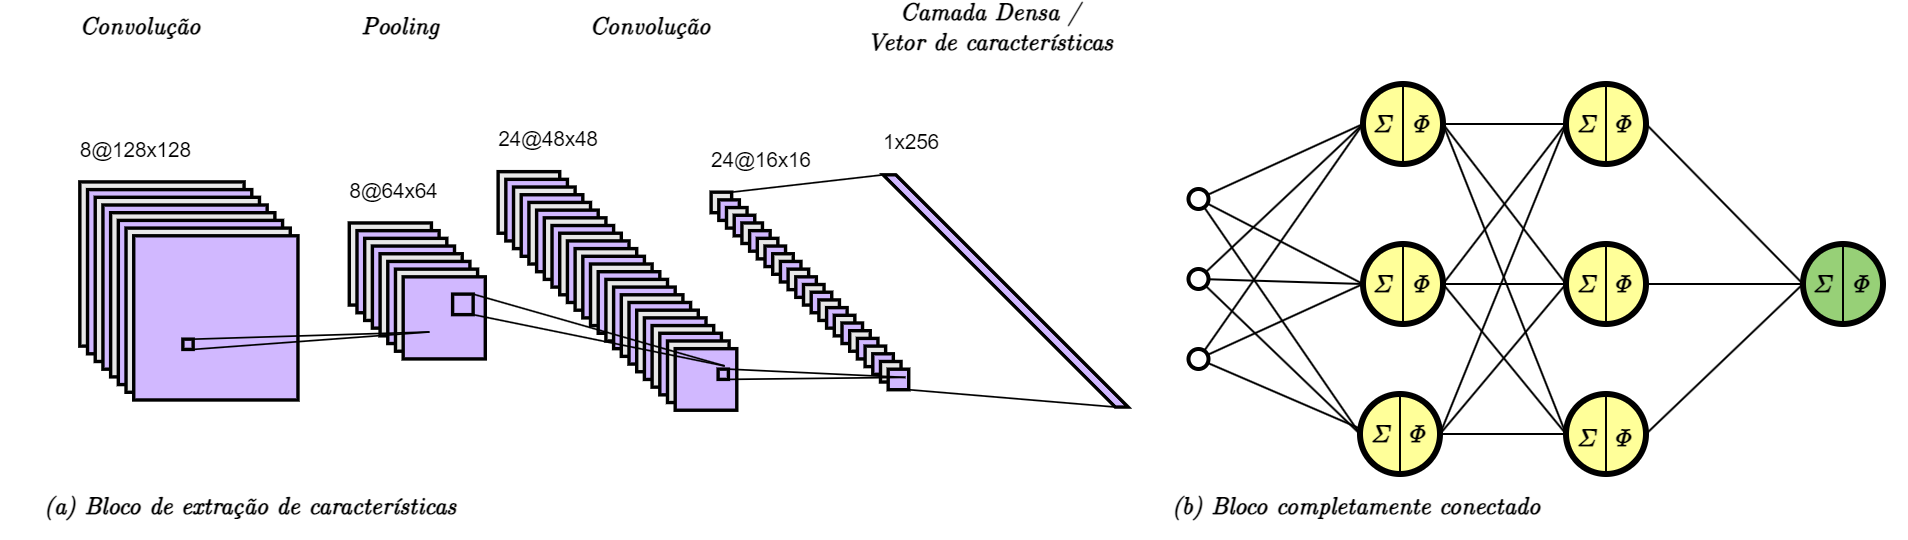
\includegraphics[scale=.23]{imagens/cnn.png}
	\label{fig:cnn}
  \source{Alexandre Farias, 2024}
\end{figure}

Uma das vantagens deste modelo é a sua capacidade de aprender características a partir de um campo receptivo da imagem, ou seja, cada neurônio pode sinalizar a importância de um conjunto de pixeis da imagem original, e não apenas de um único pixel, para a tarefa de classificação ou regressão que está sendo trabalhada. As redes neurais convolucionais

\section{Geração de dados sintéticos}

Os dados são um insumo fundamental para a pesquisa e desenvolvimento de modelos computacionais aplicados a diversas áreas do conhecimento. Recentemente, informações estruturadas como dados tabulares coletados em planilhas, imagens, vídeos e faixas de áudio, passaram a ser gerados sinteticamente com uma qualidade aceitável para sua aplicação em diferentes atividades \cite{dhariwalDiffusionModelsBeat2021}.

As motivações para geração de dados sintéticos passam pela necessidade da construção de conjuntos de dados maiores e completos, para o desenvolvimento de modelos de aprendizado de máquina, e o compartilhamento de dados sem infringir as legislações vigentes e preceitos éticos e morais sobre a privacidade, de modo a viabilizar que a comunidade científica e a indústria possam estabelecer novos avanços de tecnologia.

Neste trabalho, abordaremos as \textit{generative adversarial networks} (GANs) e os modelos de difusão (do inglês \textit{diffusion models}, DM) como técnicas empregadas para a geração de imagens sintéticas.

\subsection{Generative Adversarial Networks (GAN)}

As GANs são modelos que utilizam as redes neurais artificiais para a geração de dados sintéticos. Nesta arquitetura, duas redes neurais competem em um cenário que tem por objetivo a maximização da fidelidade dos dados gerados. Neste cenário, temos a rede que desejamos obter como rede geradora ($G$), responsável por aprender a distribuição do conjunto de dados real e gerar dados de acordo com a distribuição aprendida, e sua adversária, chamada de rede discriminadora ($D$), que tem por objetivo discriminar os dados reais dos sintéticos \cite{goodfellowDeepLearning2016}. A figura \ref{fig:gan}, ilustra de modo simplificado o cenário de treinamento de uma GAN.

\begin{figure}[htbp]
	\centering
	\caption{Diagrama de arquitetura de GAN: a rede discriminadora recebe um ruído proveniente de um espaço latente e a partir do mesmo sintetiza informações, por sua vez, a rede discriminadora recebe dados reais e sintetizados e possui como objetivo determinar a probabilidade de uma entrada ser real ou sintética.}
		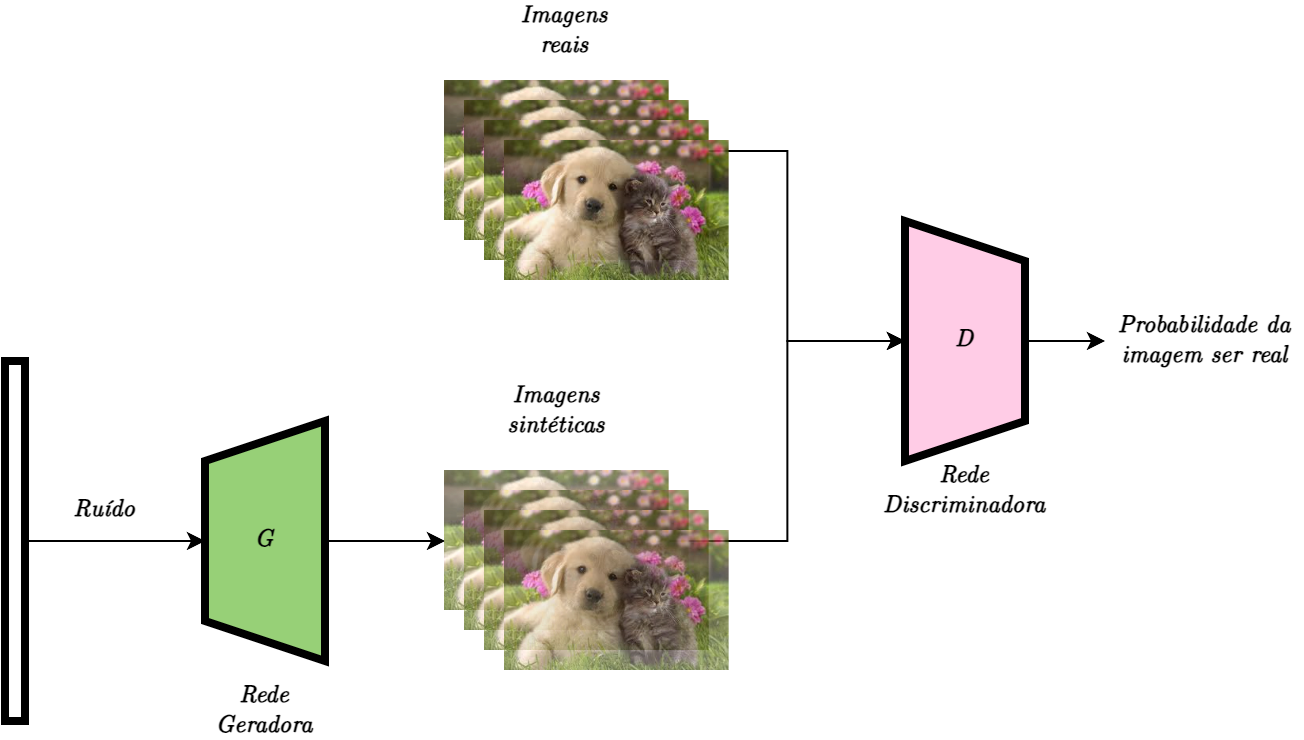
\includegraphics[scale=.25]{imagens/gan.png}
	\label{fig:gan}
  \source{Alexandre Farias, 2024}
\end{figure}

O algoritmo de aprendizado deste modelo se dá por meio de varias iterações, a cada iteração a rede $D$ é treinada mantendo-se a rede $G$ constante, após o fim da atualização dos pesos da rede $D$, na mesma iteração, a rede $G$ é atualizada de modo que aprenda com os erros de sua adversária, deste modo, finalizando uma iteração completa.

A taxa de aprendizado, ou seja, a intensidade com que os pesos são ajustados, é configurada de modo que a rede geradora possa aprender em um passo mais acelerado do que a rede discriminadora, de modo que o algoritmo possa convergir para um ponto em que a rede geradora sintetize imagens tão parecidas com as reais fazendo com que a rede discriminadora não consiga distinguir tão bem as imagens que recebe em sua camada de entrada \cite{goodfellowGenerativeAdversarialNetworks2014}.



\subsection{Difussion Models (DM)}

Os modelos de difusão (do inglês \textit{difussion models}, DM) são uma classe de modelos geradores capazes de atingir performance estado-da-arte em diversas aplicações diferentes como a síntese de imagens, vídeos e a prototipação de novas moléculas, consequentemente sendo uma ferramenta utilizada por áreas distintas como a visão computacional, processamento de linguagem natural, modelagem de séries temporais e outras aplicações interdisciplinares \cite{yangDiffusionModelsComprehensive2023}.

\begin{figure}[htbp]
	\centering
	\caption{Representação do processo de aprendizado de um modelo de difusão: em uma primeira etapa, o modelo adiciona ruído ao dado original até que ele seja destruído, já na segunda etapa por meio de uma função score o modelo gradativamente remove o ruído até obter dados verossímeis.}
		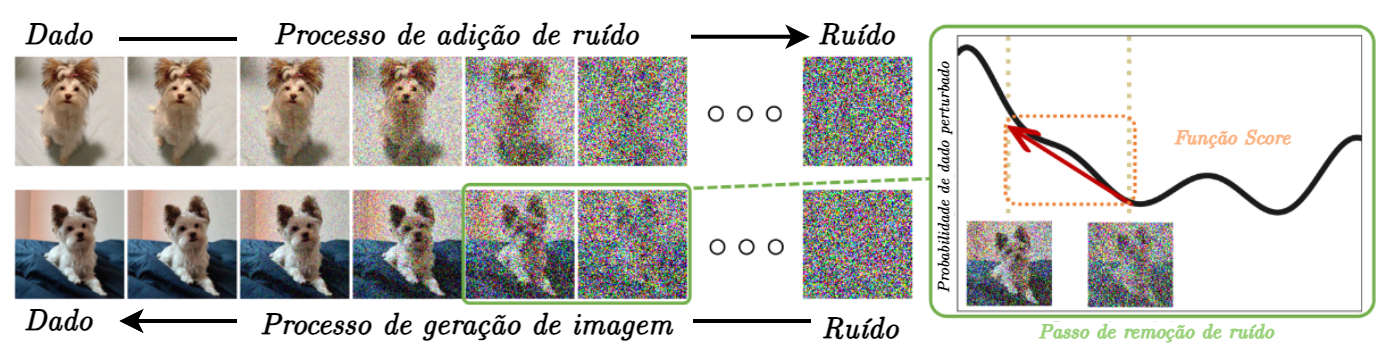
\includegraphics[scale=.28]{imagens/difussion-model.png}
	\label{fig:diffusion-model}
  \source{Adaptado de \citeonline{yangDiffusionModelsComprehensive2023}.}
\end{figure}

Estes modelos, fazem parte do paradigma de modelos generativos probabilísticos, sua abordagem envolve a adição progressiva de ruído e o aprendizado da reversão do processo de adição de ruído. De modo geral, a fase de remoção de ruído é composta por diferentes etapas, cada etapa computa os gradientes de uma função score que direcionam o processo de remoção de ruído para a construção de imagens mais prováveis e menos ruidosas, assim como ilustrado na figura \ref{fig:diffusion-model}.




\section{Explicabilidade de modelos caixa preta}